\documentclass[10pt]{article}

\usepackage[T1]{fontenc}
\usepackage[utf8]{inputenc}
\usepackage{graphicx}
\usepackage{lmodern}
\usepackage{amsmath}
\usepackage{xfrac}
\usepackage{amsthm}
\usepackage{listings}
\usepackage{enumerate}
\usepackage{amssymb}
\usepackage{cancel}
\usepackage{amsfonts}
\usepackage{float}
\usepackage{fullpage}
\usepackage{pdfpages}

\DeclareUnicodeCharacter{200A}{ }
\DeclareUnicodeCharacter{2009}{ }

\renewcommand*\contentsname{Table des matières}

\PassOptionsToPackage{hyphens}{url}\usepackage{hyperref}

\usepackage{listings}
\author{ControverSciences\textit{ et al} }
\title{Projet AREN - Corpus de ressources \\ L’éthique animale}
\date{7 Mars 2018}

\begin{document}
\maketitle

\tableofcontents

\newpage
\section{Textes à débattre}

\subsection{La cause animale est la cause de l’humanité}
\begin{itemize}
	\item \textbf{Lien : }  \url{http://www.liberation.fr/debats/2017/01/06/corine-pelluchon-la-cause-animale-est-la-cause-de-l-humanite_1539586} 
	\item \textbf{Auteur : } Propos de Corine Pelluchon, Philosophe et professeure à l’université Paris-Est-Marne-la-Vallée. Propos recueillis par Philippe Douroux.
	\item \textbf{Date : }  6 janvier 2017
	\item \textbf{Source : }  Libération, est un quotidien français dont la ligne éditoriale est de centre gauche ou de gauche sociale-démocrate.
\end{itemize}

\textbf{Pourquoi s’intéresser aux animaux en tant que philosophe ?}\\

Depuis l’Antiquité, la question animale est stratégique. Les humains se sont distingués des animaux pour cerner ce qu’ils pensaient avoir en propre : la raison, le langage articulé. Pour moi, nos rapports aux animaux sont le miroir de ce que nous sommes devenus. Le système actuel de production de la viande reflète une société fondée sur l’exploitation sans limite des autres vivants. Le profit commande la réduction constante des coûts de revient, au mépris des animaux et du sens du travail humain. La dénonciation des conditions actuelles de vie et de mort des animaux s’inscrit dans un contexte plus large, lié à la critique d’un modèle de développement générateur de contre-productivités (sur le plan social et environnemental) et à une réflexion sur ce que pourrait être une société plus juste, dans laquelle les règles ne seraient pas déterminées pour le seul bénéfice des humains et même d’une minorité de personnes. Enfin, l’exploitation des animaux dans ces conditions et à cette échelle suppose une occultation de la réalité. Si les associations de défense des animaux, comme L214 et d’autres, ne montraient pas ce qui se passe dans les élevages intensifs et les abattoirs, le public penserait que la viande est produite sans causer de souffrance. La question animale est aujourd’hui l’un des volets de la remise en question d’un système que l’on peut appeler capitaliste, à condition qu’on ne le réduise pas à l’opposition entre patronat et salariés. Fondé sur l’exploitation illimitée des autres vivants, de la nature et même des nations par d’autres nations, il dégrade l’humain. Nos rapports aux animaux révèlent ce que nous acceptons de faire à des êtres qui sont différents de nous mais qui nous ressemblent aussi beaucoup, en raison de leur sentience - c’est-à-dire de leur capacité à ressentir la douleur, le plaisir ou la souffrance.\\

\textbf{Où se trouve la limite qui veut que l’on respecte la douleur des êtres sentients ?}\\

Un être sentient ressent des émotions, la joie, la peine ou la peur, de manière subjective ; c’est un soi vulnérable, un être individué, qui vit sa vie à la première personne. Il y a quelqu’un derrière la fourrure ou les plumes. L’animal n’est pas seulement un patient moral, qui aurait des droits mais resterait passif. C’est aussi un agent moral qui peut communiquer ses préférences et ses intérêts. Les plantes ont une sensibilité, elles subissent des dommages, mais on ne peut pas en parler comme des êtres sentients - ce qui ne veut pas dire qu’on peut en faire n’importe quoi. Le rapport aux plantes est un rapport de respect : elles ont aussi une valeur non instrumentale, mais on emploie le mot «justice» à propos des êtres sentients dont les intérêts devraient entrer dans la définition du bien commun. Pour que les animaux aient des droits, il faut que les humains les formulent. Cependant, le point de départ de ces droits, ce n’est pas notre point de vue mais l’agentivité des animaux. Leur existence nous oblige et pose des limites à ce que nous pouvons faire d’eux, à nos usages des ressources.\\

\begin{flushright}
	Corine Pelluchon
\end{flushright}

\newpage
\subsection{Bien-être animal, le plus préoccupant est l’élevage en cages}
\begin{itemize}
	\item \textbf{Lien : }  \url{https://www.la-croix.com/Sciences-et-ethique/Ethique/Bien-etre-animal-preoccupant-lelevage-cages-2017-08-07-1200868238} 
	\item \textbf{Auteur : } Propos de Sophie Hild, Directrice de La Fondation Droit Animal, Éthique et Sciences et Docteure en éthologie. Propos recueillis par Frédérique Schneider
	\item \textbf{Date : }  7 août 2017
	\item \textbf{Source : }  La croix est un journal quotidien français qui se réclame ouvertement chrétien et catholique.
\end{itemize}

\textbf{Comment définir le bien-être animal ?}\\

Les animaux d’élevage ou de compagnie sont tous privés de liberté. Le prix à payer en contrepartie pour l’homme devrait être de leur offrir un environnement adapté. Car une des conditions fondamentales du bien-être animal est la possibilité d’exprimer les comportements propres à son espèce. Plus largement, le bien-être se révèle satisfaisant si les animaux sont en bonne santé physique et psychologique selon les cinq critères établis par le Farm Animal Welfare Council, en 1992 : « ne pas souffrir de la faim ou de la soif, d’inconfort, de douleurs, de blessures ou de maladie, pouvoir exprimer les comportements naturels propres à l’espèce et ne pas éprouver de peur ou de détresse ». Scientifiques, éthologues ou vétérinaires utilisent cette grille de lecture pour mesurer le bien-être animal de façon objective.\\

\textbf{Quelles sont les mesures urgentes à prendre pour respecter la nature de l’animal ?}\\

Il faut surtout se pencher sur la question de l’élevage intensif et, dans ce cadre, le plus préoccupant est l’élevage en cages, qu’il s’agisse des poules pondeuses ou des lapins. Les cages collectives des poules ont évolué en 2012, avec 750 cm2 (une feuille A4) par animal, une mangeoire d’au moins 12 cm et un abreuvoir. D’autres aménagements ont été également rendus obligatoires, comme le nid et la litière permettant le picotage et le grattage.\\

Cette nouvelle réglementation a coûté cher aux éleveurs pour un petit bénéfice pour les poules. En effet, l’animal ne peut pas exprimer de comportements normaux dans cet espace : voleter, marcher, creuser… De même, on observe des poulets qui ne tiennent plus sur leurs pattes car leurs os sont devenus trop fragiles en raison d’une sélection génétique productiviste. L’idéal pour ce type de volaille est l’élevage en plein air, sur un terrain herbagé et avec des arbres. Mais ce choix a un coût car il implique de faire évoluer les modes d’élevage. Encore aujourd’hui, 68\% de la production française d’œufs est issue de poules élevées en cages qui ne mettent jamais le nez dehors.\\

\textbf{Que dire des conditions de transport des animaux ?}\\

La réflexion sur le transport d’animaux vivants (porcs, veaux) est une urgence. Cette étape, entre l’engraissement et l’abattage, est très difficile. Ils changent d’environnement, se retrouvent dans des espaces restreints, collés à des congénères qu’ils n’ont parfois jamais vus. Cette expérience stressante donne d’ailleurs lieu à des comportements agressifs. Les organisations de protection animale, comme la nôtre, souhaitent ainsi une limitation du temps de trajet à huit heures maximum pour le bétail et moins pour la volaille. Cette mesure est relativement facile à mettre en œuvre sur le territoire français. Le plus compliqué sera le temps de trajet vers des pays tiers, sachant que la France est le premier exportateur européen d’animaux d’élevage vivants vers la Turquie (un demi-million de têtes de bétail par an).\\

\newpage
\subsection{Questionner l’expérimentation sur les animaux}
\begin{itemize}
	\item \textbf{Lien : }  \url{https://www.franceculture.fr/emissions/continent-sciences/questionner-l-experimentation-sur-les-animaux} 
	\item \textbf{Auteur : }  Stéphane Deligeorges, diplômé de philosophie, exerce différentes activités dans le milieu journalistique et littéraire.
	\item \textbf{Date : }  8 juin 2015
	\item \textbf{Source : }  Continent sciences est une émission de France Culture qui questionne le fondement de la démarche scientifique, ses ressorts, ses motivations, quelle que soit la discipline avec chaque semaine un entretien avec un chercheur différent.
\end{itemize}

Ce sont 12 millions d’animaux qui, par an et en Europe, sont utilisés dans les labos privés et publics à des fins de recherche. Que nous apprennent ces pratiques ? Sont-elles justifiables ?\\

Nous partageons l’ordinaire de nos vies avec les animaux. Par choix. Avec les chiens et les chats qui habitent nos maisons. De fait. Avec les insectes, les pigeons, les rats et même avec les renards qui résident dans certaines de nos villes. Peut-on oublier ceux que nous mangeons, ceux dont nous revêtons la peau ? Ceux-là rentrent dans le cadre d’une pratique à grande échelle. L’élevage industriel et son cortège d’abomination, de souffrance animale. Il existe, enfin, un autre univers : celui des animaux exploités. Celui sur lesquels sont testés les produits d’entretien, les cosmétiques et les médicaments qui nous soignent. C’est le monde de l’expérimentation animale. Les chiffres qui la concernent sont comme vertigineux. Ce sont 12 millions d’animaux qui, par an et en Europe, sont utilisés dans les labos privés et publics à des fins de recherche. 2,2 millions le sont en France.\\

 C’est cette expérimentation animale que nous interrogeons aujourd’hui. Que nous apprennent ces pratiques ? Sont-elles justifiables ? Justes ? Est-il possible, par d’autres méthodes, d’en faire l’économie ? Nos poussons notre enquête dans le cadre général suivant : pourquoi la reconnaissance, par le droit, du caractère sensible des animaux provoque-t-elle de tels débats ?
\newpage
\subsection{Le retour du débat sur l'expérimentation animale}
\begin{itemize}
	\item \textbf{Lien : }  \url{http://www.bfmtv.com/societe/a-l-approche-du-telethon-le-retour-du-debat-sur-l-experimentation-animale-1321647.html} 
	\item \textbf{Date : }  12 décembre 2017
	\item \textbf{Source : }  L’Agence France-Presse (AFP) est une agence de presse mondiale et généraliste chargée de collecter, vérifier, recouper et diffuser l'information, sous une forme neutre, fiable et utilisable directement par tous types de médias.
\end{itemize}



Souffrances évitables, dénoncent les uns. Étape obligée dans la quête de traitements, répliquent les autres. Le débat sur l'expérimentation animale fait rage entre militants aux vidéos choc et chercheurs qui déplorent des "caricatures". "On ne fait pas ça pour le plaisir, les scientifiques ne font pas joujou avec les animaux", assure Caroline Le Guiner, experte en thérapie génique du muscle. \\

"La liste est longue des découvertes et progrès médicaux que nous devons aux modèles animaux (récompensés par 79 prix Nobel de médecine)", rappelle un groupe de scientifiques, qui fustigent "certains groupuscules déguisés en lanceurs d'alerte". Si elle n'est pas nommée, c'est l'association Animal Testing qui est visée. Depuis un an, elle a publié trois vidéos en caméra cachée montrant des expériences en laboratoire sur des souris, des singes et des chiens.\\

"Certains rongeurs décèdent de leurs souffrances ou perdent leurs yeux", explique l'une des responsables de l'association. "Les primates sont dans des sous-sols sans lumière, dans des cages d'un mètre cube, à perpétuité", s'insurge-t-elle. "C'est pire que des conditions carcérales, certains deviennent fous en plus de leurs souffrances physiques". Ces dernières années, au fur et à mesure que montaient les préoccupations liées au bien-être animal, ces expérimentations ont été davantage encadrées. \\

Une directive européenne, transposée en droit français en 2013, met en avant le principe des "3R": remplacer (le recours aux animaux par d'autres méthodes quand c'est possible), réduire (le nombre d'animaux nécessaires à une étude), raffiner (c'est-à-dire diminuer les contraintes imposées aux animaux). Les projets utilisant des animaux doivent être examinés par des comités d'éthique et autorisés par le ministère de la Recherche.
Selon les derniers chiffres du ministère, 1,9 million d'animaux ont servi à la recherche scientifique en 2015 en France, à 71\% pour des produits et appareils médicaux, mais aussi pour la sécurité alimentaire ou l'industrie chimique. Seules les expérimentations terminées sont prises en compte. L'animal le plus utilisé est la souris (52,9\%), suivie des poissons (22,2\%), du rat (8,2\%) et du lapin (5,6\%). Les chiens (3.226 spécimens) et les primates (3.162, dont 90\% de macaques) représentent moins de 0,2\% chacun.\\

Les chercheurs ont restauré la force musculaire de chiens atteints de la myopathie de Duchenne et stabilisé leurs symptômes grâce à une thérapie génique innovante. Une première encourageante dans la perspective, encore lointaine, d'un traitement chez l'humain. Les douze golden retrievers étaient naturellement malades. À partir d'un spécimen initial, une colonie a été créée par reproduction. Sans ces chiens, ces travaux complexes n'auraient pas été possibles, souligne la chercheuse: "C'est une étape obligée (...). Tout est très encadré et le but est d'avoir un jour des médicaments pour les enfants" atteints de cette maladie génétique, dont l'espérance de vie ne dépasse pas en moyenne les 30 ans.\\


\newpage

\section{Corpus de ressources}

\subsection{Peut-on se passer des modèles animaux ?}

\begin{itemize}
	\item \textbf{Lien : }  \url{https://lejournal.cnrs.fr/articles/peut-se-passer-des-modeles-animaux} 
	\item \textbf{Auteur : } Yaroslav Pigenet, journaliste scientifique.
	\item \textbf{Date : } 26 octobre 2017
	\item \textbf{Description : } Contribution majeure aux progrès de la biologie et de la médecine, l’expérimentation animale reste la cible de critiques, malgré un encadrement de plus en plus strict.
	\item \textbf{Source : } CNRS Le journal a pour objectif de partager largement avec les amateurs de science, les professeurs et leurs élèves, les étudiants et tous les citoyens curieux, des contenus destinés jusque-là à la communauté des agents du CNRS, chercheurs, ingénieurs et techniciens, ceux des labos comme ceux des bureaux.
\end{itemize}

Dans son Traité de la maladie sacrée, Hippocrate écrivait à propos de l’épilepsie : « On peut reconnaître la vérité de ceci sur les brebis, qui sont sujettes à être attaquées de cette maladie, et surtout sur les chèvres chez qui elle est très fréquente. Si on ouvre la tête d’une chèvre, on trouve le cerveau humide, plein d’eau et exhalant une mauvaise odeur. D’où il ressort évidemment que ce n’est pas un dieu qui afflige ici le corps, mais bien la maladie. Il en est de même pour l’homme. » Celui que l’on considère comme le père de la médecine était ainsi le premier à décrire et utiliser un modèle animal pour observer et tenter d’expliquer les causes physiques d’une maladie humaine qu’on pensait d’origine surnaturelle. Il faudra attendre la naissance du clone Dolly pour que le modèle brebis retrouve brièvement la faveur des chercheurs, mais 2 500 ans plus tard, cette méthode d’investigation et d’observation des organismes vivants demeure l’un des piliers de la recherche biologique et médicale contemporaine : les modèles animaux ont été à l’origine de plus de 70 prix Nobel, et de la plupart des avancées biomédicales des 150 dernières années. Cela va du modèle du lapin qui a permis à Pasteur d’inventer le vaccin contre la rage, à celui de la mouche drosophile grâce auquel Jules Hoffmann, prix Nobel 2011, a dévoilé les mécanismes de l’immunité innée, en passant par le modèle du rat avec lequel John O’Keefe, May-Britt Moser et Edvard Moser, nobélisés en 2014, ont compris comment le cerveau traite l’information spatiale.\\

\textbf{L’instauration d’un cadre}\\

Toutefois, s’ils ont connu un essor extraordinaire depuis la Seconde Guerre mondiale, ces modèles ont également montré certaines limites, et de plus en plus de voix se sont élevées pour condamner l’exploitation irraisonnée des animaux et réclamer une meilleure prise en compte de leur souffrance. Bien avant que cette demande ne prenne de l’ampleur, la communauté scientifique a tenté d’y répondre en établissant dès la fin des années 1950 une règle visant à réduire au strict minimum le recours aux animaux.\\

C’est d’ailleurs dans ce cadre philosophique et sous la pression grandissante du public que les législateurs ont élaboré depuis une trentaine d’années de nouvelles lois, directives et recommandations éthiques encadrant de plus en plus sévèrement le recours à l’animal dans la recherche, fixant même comme objectif ultime le remplacement de toute expérimentation sur les vertébrés par des méthodes substitutives. Un but que la plupart des chercheurs n’estiment toutefois pas réaliste, même à long terme, si ce n’est au prix d’un ralentissement sensible des progrès de la recherche biomédicale et d’une diminution drastique de la sécurité sanitaire.\\

Avec les études sur les tissus, les cellules et les molécules biologiques, l’utilisation des modèles animaux fait partie des principaux outils à la disposition du biologiste pour interroger et comprendre le vivant. Elle seule permet d’étudier les réponses intégrées d’un organisme ainsi que les interactions entre cellules, tissus et organes qui le composent. Elle seule permet aussi, sans recourir à l’expérimentation sur l’homme, d’analyser les causes des maladies, d’envisager des traitements et d’en tester l’efficacité. Au fondement de toute expérimentation animale, il y a un organisme qui va servir de modèle à un autre, plus sensible, moins accessible ou plus difficilement manipulable.\\

 « Du point de vue scientifique, on choisit un modèle animal selon trois critères principaux : d’abord la similitude du modèle avec les caractéristiques du phénomène étudié chez l’espèce cible – souvent l’homme –, ensuite, en recherche biomédicale, le degré de similitude entre le mécanisme biologique de la maladie humaine étudiée et celui du modèle lui-même, enfin en recherche préclinique, la similitude des réponses à un traitement pharmacologique, explique le généticien Yann Hérault. Un modèle animal est aussi la résultante d’un ensemble de données génétiques, de l’interaction de son génome avec l’environnement dans lequel il est étudié et des approches méthodologiques mises en œuvre pour l’analyser. »\\
 
\textbf{ La spécialisation des modèles}\\
 
 À partir des années 1950, l’expansion de la recherche biomédicale va en effet aller de pair avec la multiplication et la spécialisation des modèles animaux, débouchant sur des avancées majeures dans tous les domaines de la biologie, tant fondamentaux qu’appliqués. Au modèle brebis d’Hippocrate vont ainsi s’ajouter la souris, le lapin, le rat, le poulet, le poisson zèbre, le macaque, etc., ainsi que les superstars des modèles invertébrés : la mouche drosophile et le ver nématode.\\
 
 La place des modèles animaux dans les sciences biologiques et médicales ne va cesser de s’accroître tout au long du xxe siècle, le nombre d’articles scientifiques y faisant référence atteignant un record au cours des années 1990. D’autant qu’en plus de s’être diversifiés et spécialisés, ces modèles ont connu récemment une évolution majeure avec l’usage d’animaux génétiquement édités, grâce auxquels des variations génétiques fines permettent de modéliser encore plus précisément des mécanismes physiopathologiques de plus en plus nombreux. On peut citer l’exemple de ces souris génétiquement modifiées de manière à ce qu’elles puissent être infectées par la bactérie listeria, fournissant un modèle pour étudier la listériose humaine.\\
 
 Cette spécialisation des modèles a poussé les chercheurs à créer des banques d’animaux modèles. « Principalement constituées de gamètes ou d’œufs congelés, ces banques contiennent des modèles animaux de référence, possédant des caractéristiques phénotypiques et génétiques bien définies et déjà décrites dans la littérature scientifique, précise Yann Hérault, qui a été directeur du laboratoire Transgenèse et archivage d’animaux modèles, à Orléans. Elles permettent, en les conservant dans des bases de données informatiques interrogeables à distance, de garantir la préservation des caractéristiques génétiques et des informations zootechniques sur ces modèles, ainsi que de les rendre largement accessibles à la communauté scientifique. »
 
\textbf{ Entre épistémologie et éthique}\\
 
 Reste qu’en dépit de sa contribution incomparable aux progrès de la biologie et de la médecine, le recours aux modèles animaux est désormais la cible de critiques de plus en plus virulentes, tant sur le plan épistémologique qu’éthique. « La biologie moderne s’est construite sur le constat de l’unité du vivant. Le fait que nos gènes possèdent 60\% d’homologie avec ceux de la mouche drosophile et 90\% avec ceux de la souris nous a permis, grâce à l’expérimentation animale, d’élucider plusieurs mécanismes physiologiques fondamentaux et certaines pathologies, mais il reste délicat de postuler que ce qui se passe dans le cerveau d’un poisson ou d’un rongeur modélise parfaitement tout ce qui se passe dans celui d’un humain ; ainsi le recours à des primates modèles est parfois indispensable pour étudier des processus neurobiologiques ou comportementaux complexes, explique le chercheur Jean-Stéphane Joly. Devant le nombre de plus en plus grand d’organismes modèles à sa disposition, le biologiste se doit aujourd’hui de bien s’interroger sur la pertinence de celui ou ceux qu’il va choisir pour répondre à la question qu’il se pose. » Toutefois, bien plus que les interrogations sur la validité et la valeur prédictive des modèles animaux, ce sont celles concernant le statut et le bien-être de l’animal qui, trouvant un écho croissant auprès de la population, ont fini par mettre l’expérimentation animale sur la sellette.\\
 
\textbf{ Des méthodes substitutives}\\
 
 La communauté scientifique n’a d’ailleurs pas attendu que le grand public et le législateur s’y intéressent pour réfléchir aux problèmes éthiques posés par l’expérimentation animale et à l’élaboration de méthodes alternatives. Ainsi, dans leur ouvrage The Principles of Humane Experimental Technique, William Russell et Rex Burch ont défini dès 1959 la règle dite « des 3 R ». Celle-ci consiste à développer et à favoriser les méthodes d’investigation pouvant se substituer à l’utilisation de l’animal (Replacement, substitution en français), mais aussi celles capables de réduire le nombre d’animaux utilisés (Reduction) ou encore de diminuer la douleur ou le stress imposés à ces animaux (Refinement, raffinement ou amélioration en français). Cette philosophie des 3 R va de fait servir de cadre à la communauté scientifique, mais également inspirer la plupart des recommandations éthiques, règlements et lois élaborés depuis pour réguler le recours à l’expérimentation animale.\\
 
 Dans les 3 R, le premier R désigne donc les méthodes qui évitent l’utilisation d’une espèce animale donnée dans un domaine où elle était jusqu’alors nécessaire. Cette substitution peut consister en un remplacement d’animaux vertébrés, dont la sensibilité est considérée comme élevée, par des animaux dont le potentiel de perception de la douleur est réputé moins grand, comme certains invertébrés notamment.\\
 
 « Pour les remplacements “complets” d’animaux, on peut par exemple envisager des méthodes d’investigation passant par un dispositif in vitro faisant interagir des éléments biologiques comme les tissus, les cellules, les organites, les biomolécules, ou par un dispositif ex vivo constitué d’un organe bio-artificiel (aussi appelé organoïde) obtenu à partir de cultures de cellules-souches, ou bien encore par des dispositifs in silico ou organ-on-a-chip réalisant des simulations bio-informatiques basées sur la modélisation mathématique des données biologiques », indique Jean-Stéphane Joly.\\
 
  Les outils de ce type se multiplient, tel l’I-Wire, un système bioélectronique qui permet d’étudier les propriétés biomécaniques du cœur humain. Composé d’un fil de cellules tendu entre deux supports sensibles, l’appareil réagit à certains médicaments de la même façon que le font les cellules du cœur. Grâce à ce système, les chercheurs espèrent mieux connaître l’effet du stress sur le cœur sans recours aux êtres vivants. « Les progrès potentiels sont importants, mais je préfère le terme de méthodes complémentaires à celui d’alternatives car, même quand elles seront parfaitement au point – et elles ne le sont pas encore –, aucune ne sera en mesure de fournir les réponses qu’apporte aujourd’hui l’expérimentation sur des organismes entiers, tempère le chercheur. Ces méthodes pourront en revanche être combinées dans des approches intégratives combinant in vitro, ex vivo et in silico où l’animal ne sera utilisé qu’en dernier recours, lorsque les “alternatives” n’auront pas permis d’apporter les informations suffisantes. »\\
 
 À ce titre, les méthodes de « substitution » s’apparentent de facto aux méthodes de réduction, le deuxième R, dont le but est de réduire le nombre d’animaux utilisés dans les études plutôt que de les éliminer complètement. « Ces méthodes de réduction sont déjà largement mises en œuvre dans nos laboratoires, rappelle le vétérinaire Ivan Balansard, délégué scientifique au bureau éthique et modèles animaux du CNRS. Elles consistent en particulier à concevoir des plans d’expérience plus efficaces ainsi que des tests statistiques plus pertinents, qui vont permettre d’obtenir des résultats significatifs sur des effectifs réduits. Elles passent aussi par le partage de banques de données de résultats expérimentaux, la création de centres de ressources d’animaux modèles au génome ou au phénotype bien établi, ainsi que par la réutilisation d’animaux. » On notera que, par la quantité inédite d’informations qu’il permet de recueillir, l’essor récent des techniques « omiques » de mesure à haut débit du matériel génétique ou des protéines permet, lui aussi, un usage plus parcimonieux des animaux.\\
 
 \newpage
 
\textbf{ Diminuer stress et douleurs}\\
 
 Enfin, les méthodes relevant du troisième R (Refinement, soit amélioration) désignent les modifications apportées aux conditions d’élevage ainsi qu’aux procédures expérimentales et d’observation dans le but de réduire le stress et la douleur des animaux utilisés. Elles se traduisent par exemple par l’utilisation de techniques d’exploration non invasives telles que l’imagerie RMN, la télémétrie, le recours systématique à l’anesthésie, l’évaluation comportementale, notamment. Ce sont également toutes les bonnes pratiques de zootechnie qui améliorent la vie des animaux tout en augmentant la validité des modèles.
 
  En France, les deux premiers R sont inscrits dans le Code rural depuis 1987. Celui-ci a été complété en 2013 par six décrets transposant la directive européenne 2010/63/UE, qui établit la règle des 3 R comme cadre de toute recherche animale. Ainsi, cette réglementation protège tous les vertébrés (et les céphalopodes), dont elle régule les conditions d’élevage, et soumet toute utilisation d’animaux à l’approbation d’un comité d’éthique agréé. Elle ne s’applique toutefois pas aux autres invertébrés comme les insectes. Elle restreint par ailleurs fortement le recours aux primates modèles et aux carnivores (chiens, chats et furets) et interdit l’utilisation des grands singes.\\
  
\textbf{ Des personnels bien formés}\\
 
 Ces nouvelles règles ont été parfaitement intégrées par la communauté scientifique. « En France, et plus généralement en Europe, la recherche animale repose sur des personnels bien formés dans des structures réglementées, s’efforçant d’utiliser les méthodes les moins invasives possible, avec des protocoles standardisés, robustes, reproductibles et surtout respectueux du bien-être animal, de l’éthique et plaçant la règle des 3 R au centre de leur réflexion, témoigne Yann Hérault. De plus en plus de protocoles sont organisés en batterie, donnant un tableau clinique basé sur plus de 200 paramètres physiologiques et comportementaux pour chaque individu, en minimisant le mal-être, en affinant les méthodes et en réduisant le nombre d’animaux étudiés. »\\
 
  Ces progrès et ces réglementations sont néanmoins jugés insuffisants par une partie du public. L’initiative citoyenne européenne (ICE) « Stop Vivisection », prônant notamment l’interdiction de toute expérimentation sur l’animal au profit de méthodes substitutives, a été lancée en 2012 et signée par 1,17 million de citoyens de l’UE. Outre la guérilla que mènent certains activistes contre les centres de recherche animale, les scientifiques supportent assez mal le procès d’intention qui leur est fait quant à leur supposée indifférence au bien-être animal. « Nous ne sommes ni des sadiques, ni des robots, souligne Guillaume Masson, directeur du Centre d’exploitation fonctionnelle et de formation en primatologie. Quand on travaille quasi quotidiennement avec un groupe de macaques pendant plusieurs mois voire années, on s’attache fortement à eux, on fait tout pour leur rendre la vie pas seulement supportable, mais agréable, comme le ferait un maître aimant pour son compagnon animal. » Et quoiqu’ils comprennent et acceptent la multiplication des contrôles encadrant l’expérimentation, certains chercheurs s’interrogent sur les priorités du législateur. « Nous respectons scrupuleusement toutes les règles européennes et françaises dans nos expériences sur les poissons zèbres, pointe la généticienne Laure Bally-Cuif, directrice adjointe du laboratoire Bases génétiques, moléculaires et cellulaires du développement. Je note cependant qu’en Europe, aujourd’hui, la qualité de vie d’un poisson zèbre en laboratoire fait l’objet d’infiniment plus d’attention que celle des milliers de poissons qui finissent asphyxiés ou mutilés dans les filets de la pêche industrielle. »\\
  
\textbf{ L’inquiétude des chercheurs}\\
 
 Dans la réponse qu’elle a publiée en 2015 à l’ICE « Stop Vivisection », la Commission européenne jugeait prématuré un bannissement immédiat, mais elle concédait « partager la conviction que l’expérimentation animale doit être progressivement supprimée en Europe ». Une position qui inquiète beaucoup les chercheurs, car peu d’entre eux croient qu’on pourra un jour, même à long terme, se passer totalement des études sur les modèles animaux.\\
 
 En réalité, l’interdiction complète des tests sur l’animal est déjà appliquée en Europe depuis 2009 dans le domaine des produits cosmétiques, et cela pourrait un jour poser problème : « En cosmétologie, les tests peuvent être pratiqués sur des cultures isolées de peau humaine – la technique est assez bien maîtrisée –, mais il faut savoir que cette peau bio-artificielle ne comporte ni poils, ni terminaisons nerveuses, ni vaisseaux sanguins, bref rien de tout ce qui fait de la peau un organe et pas un simple tissu, insiste Jean-Stéphane Joly. Ainsi, les tests pratiqués vont pouvoir nous dire si tel ou tel produit est irritant ou localement cancérigène, mais nous ne saurons pas si d’éventuelles nanoparticules entrant dans sa composition peuvent gagner la circulation sanguine et interférer avec notre système immunitaire. » \\
 
 Dans le développement de nouveaux médicaments, renoncer à l’expérimentation sur un ou plusieurs modèles animaux revient à reporter le risque sur l’être humain. Le scandale de la thalidomide, cet anti-nauséeux prescrit dans les années 1950 aux femmes enceintes et qui a entraîné la naissance de dizaines de milliers d’enfants malformés, illustre dramatiquement ce risque. La molécule avait été testée sur des rates gravides, sans qu’aucun effet tératogène ne soit détecté. Or, la thalidomide n’est pas métabolisée de la même manière par les rongeurs et par les primates. « Il faut se méfier de la facilité du modèle animal unique et généraliste, prévient Ivan Balansard. On viole aussi l’éthique en utilisant un modèle inadéquat ! »\\
 
 Depuis le désastre de la thalidomide, le recours à une espèce « non-rongeur » est devenu obligatoire dans les essais précliniques des médicaments. « La difficulté est la même pour la recherche fondamentale, où se restreindre à l’étude des molécules, des cellules et des tissus risque de freiner – si ce n’est de stopper – tout progrès dans notre compréhension de la mécanique et des interactions complexes entre constituants qui caractérisent tout organisme vivant, poursuit le chercheur. Même si de nouvelles approches et des méthodes d’exploration révolutionnaires émergent, l’utilisation de modèles animaux demeurera encore longtemps indispensable au progrès scientifique et médical. La recherche biologique en a besoin car c’est tout simplement le seul moyen dont nous disposons pour observer et comprendre le fonctionnement de l’organisme et des grandes maladies systémiques comme le cancer. Bien entendu, cette recherche doit se faire dans le plus grand respect des règles d’éthique et de bien-être animal. »
\newpage 

\subsection{Cinq scénarios pour imaginer le futur des relations entre l’homme et l’animal}
\begin{itemize}
	\item \textbf{Lien : }  \url{https://theconversation.com/cinq-scenarios-pour-imaginer-le-futur-des-relations-entre-lhomme-et-lanimal-70792} 
	\item \textbf{Auteur : } Anne-Laure Thessard, Doctorante en sémiotique à l'Université Paris-Sorbonne
	\item \textbf{Date : } 2 janvier 2017
	\item \textbf{Source : } The Conversation France est un média en ligne d'information et d'analyse de l'actualité indépendant, qui publie des articles grand public écrits par les chercheurs et les universitaires. 
\end{itemize}



Au sein de la technosphère contemporaine, l’impact des activités humaines sur la nature intensifie et complexifie les rapports que l’humain entretient avec la nature et les animaux ; l’existence de ces derniers est ainsi économiquement, écologiquement et techniquement assujettie au traitement que leur réservent les êtres humains. \\

Dans ce contexte toujours plus mécanisé, les maltraitances et les violences commises principalement sur les animaux de rente ont récemment fait l’objet d’un écho inédit avec la mobilisation d’associations comme L214 ou Peta.\\

En fait, qu’il s’agisse d’animaux sauvages, de rente ou de compagnie, la question de la frontière entre les espèces et de la valeur de l’animal – « outil » ou « être à part entière » – mobilise de plus en plus l’opinion.\\

En décembre dernier, un rapport ministériel de prospective paraissait, proposant cinq scénarios au sujet de l’évolution du rapport entre humains et animaux à l’horizon 2030. Au sujet de l’animal, ce rapport spécifie que « son devenir est incertain car les sources d’inflexion sont nombreuses ».\\

Ces trois principaux facteurs d’inflexion concernent le contexte économique, la situation écologique et l'évolution des représentations humaines à l’égard des animaux. 
Trois questions parcourent ainsi l’ensemble du rapport : le rapport homme-animal deviendra-t-il l’un des enjeux structurants de la société française, de son système alimentaire, et des évolutions du monde agricole et rural ? Sera-t-il au contraire un thème marginal, subordonné à d'autres facteurs plus déterminants ? Sa mise en débat et sa gestion seront-elles pacifiées ou conflictuelles ?\\

\textbf{Scénario 1 : la sobriété forcée}\\

Dans ce premier scénario, les animaux subissent moins de mauvais traitements dans le but d’optimiser leur exploitation. L’animal est ainsi toujours conçu comme outil, déterminé par l’usage humain et est envisagé comme « solution écologique, pratique, et surtout peu onéreuse ».\\

Dans ce contexte économique contraint où les microfilières se développent, « les mouvements les plus radicaux, positionnés sur la dénonciation de toute forme d’exploitation animale, perdent en audience ». Les microfilières assurent auprès du public de « garantir le respect animal en abattoir » et promeuvent la pratique de la « ferme ouverte ». En outre, la contrainte économique alliée à la nécessité du maintien de la biodiversité réduisent la préoccupation vis-à-vis des animaux à quelques « animaux-symboles ».\\

Dans ce scénario de « sobriété forcée », l’animal demeure une ressource, c’est-à-dire un outil pour l’être humain : il est une source d’alimentation, une variable d’optimisation dans la gestion de l’environnement et un compagnon au statut fonctionnel.\\

\newpage

\textbf{Scénario 2 : la sobriété environnementale choisie}\\

Dans ce second scénario, l’approche de « la santé globale » (one health) qui inclue le respect de l’environnement, prévaut dans la société française. Autour des années 2020, l’opinion publique s’entend autour de l’idée que la mise à mort fait partie de « l’ordre des choses ». Suite à la correction des abus de traitements infligés aux animaux de rente, l’émotion suscitée dans le milieu des années 2010 par les thèses antispécistes s’essouffle, laissant place à une « une relégitimation de l’abattage des animaux ».\\

Dans ce contexte économique favorable, le consommateur a une plus grande incidence sur l’offre des produits de consommation. Les Français réduisent leur consommation de viande animale et souhaitent favoriser « l’agrobiodiversite ».\\

En outre, du point de vue écologique « la non-soutenabilité de la trajectoire actuelle, amène progressivement un changement du regard dominant sur la place de l’humain dans la nature ». La cohabitation entre les hommes et les animaux, mêmes sauvages à l’image du loup, est renforcée par le développement de « centres d’expérimentation de nouvelles cohabitations entre hommes et animaux sauvages », ainsi que par la diversification du compagnonnage animal (les cochons, chèvres, poules sont aussi des animaux de compagnie).\\

Dans ce scénario, bien que les animaux soient davantage intégrés à la société, ils n’ont toujours pas de droits fondamentaux et demeurent, pour certains, des ressources : « Sans acquérir le statut juridique de personne morale, les animaux voient leurs “droits” […] augmenter, quelles que soient leurs “fonctions” ».\\

\textbf{Scénario 3 : l’hypermécanisation des rapports}\\

La crainte d’attaques biologiques terroristes, l’intensification de l’élevage industriel et la dégradation écologique générale, portent l’attention sur les risques zoonotiques, et font passer la santé publique avant « les préoccupations éthiques et même économiques liées aux soins animaux ».\\

L’intensification de l’automatisation généralisée conduit à intégrer la filière agricole à des filières « bioéconomiques » plus vastes. La demande en produits agricoles poursuit sa forte hausse, bien que l’offre française soit concurrencée par des pays produisant à moindre coût. La production est réduite à quelques races d’animaux de rente dans un souci d’« d’écologie industrielle ».\\

Par ailleurs, les innovations en matière de protéine animale participent à menacer le statut des animaux de rente, qui deviennent moins intéressants économiquement et écologiquement parlant. Dans le même temps, la distinction entre les animaux de rente et les animaux de compagnie s’épaissit. Ces derniers sont en concurrence avec les robots de compagnie, dont l’usage se répand petit à petit après les années 2020. De sorte que, « les statuts juridiques accompagnent cette évolution, avec une différenciation normative fondée sur la fonction sociétale et la “destination” de l’animal ».\\

Dans ce contexte général particulièrement dégradé, les animaux sont souvent identifiés aux nuisances qu’ils peuvent occasionner. Ainsi, ils sont réduits à des « variables d’ajustement ». Pourtant, la contestation du traitement infligé aux animaux continue à revenir par vague : « A l’Assemblée nationale, le club parlementaire antispéciste, créé en 2027, parvient à mettre en débat l’abolition de la mort utilitaire, mesure qui semble pour beaucoup irréaliste mais qui témoigne d’une contestation croissante et de plus en plus agissante ».\\

\textbf{Scénario 4 : éthique et durabilité}\\

La prospérité économique permet une meilleure action écologique et une prise en compte éthique intrinsèque de l’animal. Ainsi, « les défenseurs du statu quo sont mal perçus. Le respect des animaux devient un sujet très politisé, partout où ces derniers sont “exploités” et menacés ». Globalement, l’éthique, la durabilité et la santé globale deviennent des enjeux majeurs.\\

La production est centrée sur les produits végétaux, notamment par le soutien de la Silicon Valley qui investit « dans la recherche et le développement de produits de substitution » ; et 55\% des moins de 30 ans s’orientent vers une alimentation limitant les produits d’origine animale.\\

Du point de vue écologique, « à compter de la loi biodiversité de 2023, un véritable quadrillage environnemental, limitant parfois fortement les activités humaines. […] il ravive les débats sur la place de l’homme, de la nature et de l’animal sauvage ».\\

En termes juridiques, le statut de l’animal évolue significativement. Celui de l’animal de compagnie devient proche du statut d’une personne dépendante ; celui des animaux d’élevage et des animaux sauvages suit la même dynamique ; l’expérimentation animale est abolie au profit du développement d’alternatives telle l’expérimentation sur tissus in vitro (ce qui délocalise certains domaines de la recherche pour lesquels le modèle animal ne peut pas encore être remplacé).\\

Dans ce contexte favorable à une modification du modèle économique agricole en faveur de la production massive de produits végétaux (bien que certains rares animaux – en races et en nombre – continuent à être élevés pour être consommés), l’animal d’élevage est « exfiltré » de la société. Paradoxalement, cette configuration donne l’opportunité de penser des droits pour les animaux, en dehors de toute fonction préconçue.\\

\textbf{Scénario 5 : prospérité et indifférence}\\

Dans ce dernier scénario favorable économiquement, l’individualisme et les choix utilitaristes priment sur toute considération éthique et ce dans tous les domaines : « Les logiques sectorielles (économiques, sanitaires, écologiques, etc.) s’autonomisent, dans une réelle indifférence du public ». Courant 2030, la question alimentaire est sortie du débat public.\\

Économiquement parlant, dans cette logique individualiste et sectorielle cohabitent différentes communautés alimentaires basées sur les protéines végétales, les insectes et la viande in vitro. La consommation de viande animale persiste, via des élevages intensifs ou des circuits courts.\\

Dans le même ordre d’idée, la logique du soin globale (one health) implique un soin envers les animaux, uniquement dans la mesure où cela dépend de la sécurité sanitaire humaine ou que des impératifs économiques l’imposent.\\

Dans ce contexte centré sur l’individu : « Des innovations en robotique concurrencent puis limitent les interactions directes homme-animal ». L’indifférence généralisée implique un statu quo par rapport aux droits des animaux : « Pour la plupart des Français, l’attachement à leur animal de compagnie coexiste avec une certaine indifférence à l’égard des autres animaux ».\\

\textbf{Un choix de société}

Dans ces cinq scénarios de « futurs possibles » se dessine en filigrane une alternative : les animaux devraient-ils être conçus comme de purs outils et ressources exploitables ou bien pensés dans leur valeur intrinsèque ?\\

Dans un contexte d’hypermécanisation où les animaux d’élevage sont principalement traités comme des outils – et leurs besoins physiologiques primaires non respectés –, la question de la valeur intrinsèque de la vie des animaux s’impose plus clairement encore. Ce qui serait peut-être moins le cas dans une configuration économique d’élevage traditionnel, pour laquelle les conditions de vie élémentaire sont davantage respectées et permettent de laisser au second plan la question de la valeur intrinsèque de la vie animale.\\

La production intensive de produits d’origine animale polarise donc le questionnement contemporain sur la condition animale autour de l’alternative entre les « animaux outils » et les « animaux conçus pour leur valeur intrinsèque ».\\

Cette polarisation met la société en face d’un choix qui n’est plus seulement utilitaire, à savoir bien traiter les animaux destinés à la consommation humaine, ou poursuivre des mauvais traitements qui peuvent avoir un impact sur la santé humaine et sur l’environnement. La question animale prend une dimension éthique également centrée sur la valeur de la vie animale. En effet, est-il soutenable éthiquement et écologiquement de maintenir des processus et des pratiques violentes au regard du respect des êtres vivants ? Et si le respect des animaux est une question légitime, comment ne pas envisager des droits empêchant toute forme de violence subie par les animaux ? Par extension, si l’évolution des droits pour les animaux est légitime, condamner toute forme de maltraitance et de violence envers les animaux, ne passe-t-il pas par la promulgation de droits fondamentaux ?\\

C’est bien souvent la configuration économique et, dorénavant, écologique qui permet de statuer sur ces questions de représentation du vivant en général. Cela dit, le statut de l’animal et sa valeur intrinsèque sont des sujets qui intéressent de plus en plus l’opinion publique. Et si cet intérêt semble moins mesurable, il peut cependant jouer un rôle significatif et fondamental dans l’évolution de la société, des mœurs, dans la gestion économique et écologique, relatifs à la question animale, et plus généralement dans le rapport entre les humains et les animaux.


\subsection{L'éthique animale, entre science et droit}
\begin{itemize}
	\item \textbf{Lien : }  \url{https://www.pourlascience.fr/sd/science-societe/lethique-animale-entre-science-et-droit-7928.php} 
	\item \textbf{Auteur : } Georges Chapouthier est un neurobiologiste et un philosophe, il est directeur de recherche émérite au CNRS.
	\item \textbf{Date : } 23 mai 2014
	\item \textbf{Source : } Pour La Science est la version française du mensuel Scientific American. C'est une revue de vulgarisation scientifique dans toutes les disciplines, dont les articles sont signés par les chercheurs eux-mêmes.
\end{itemize}

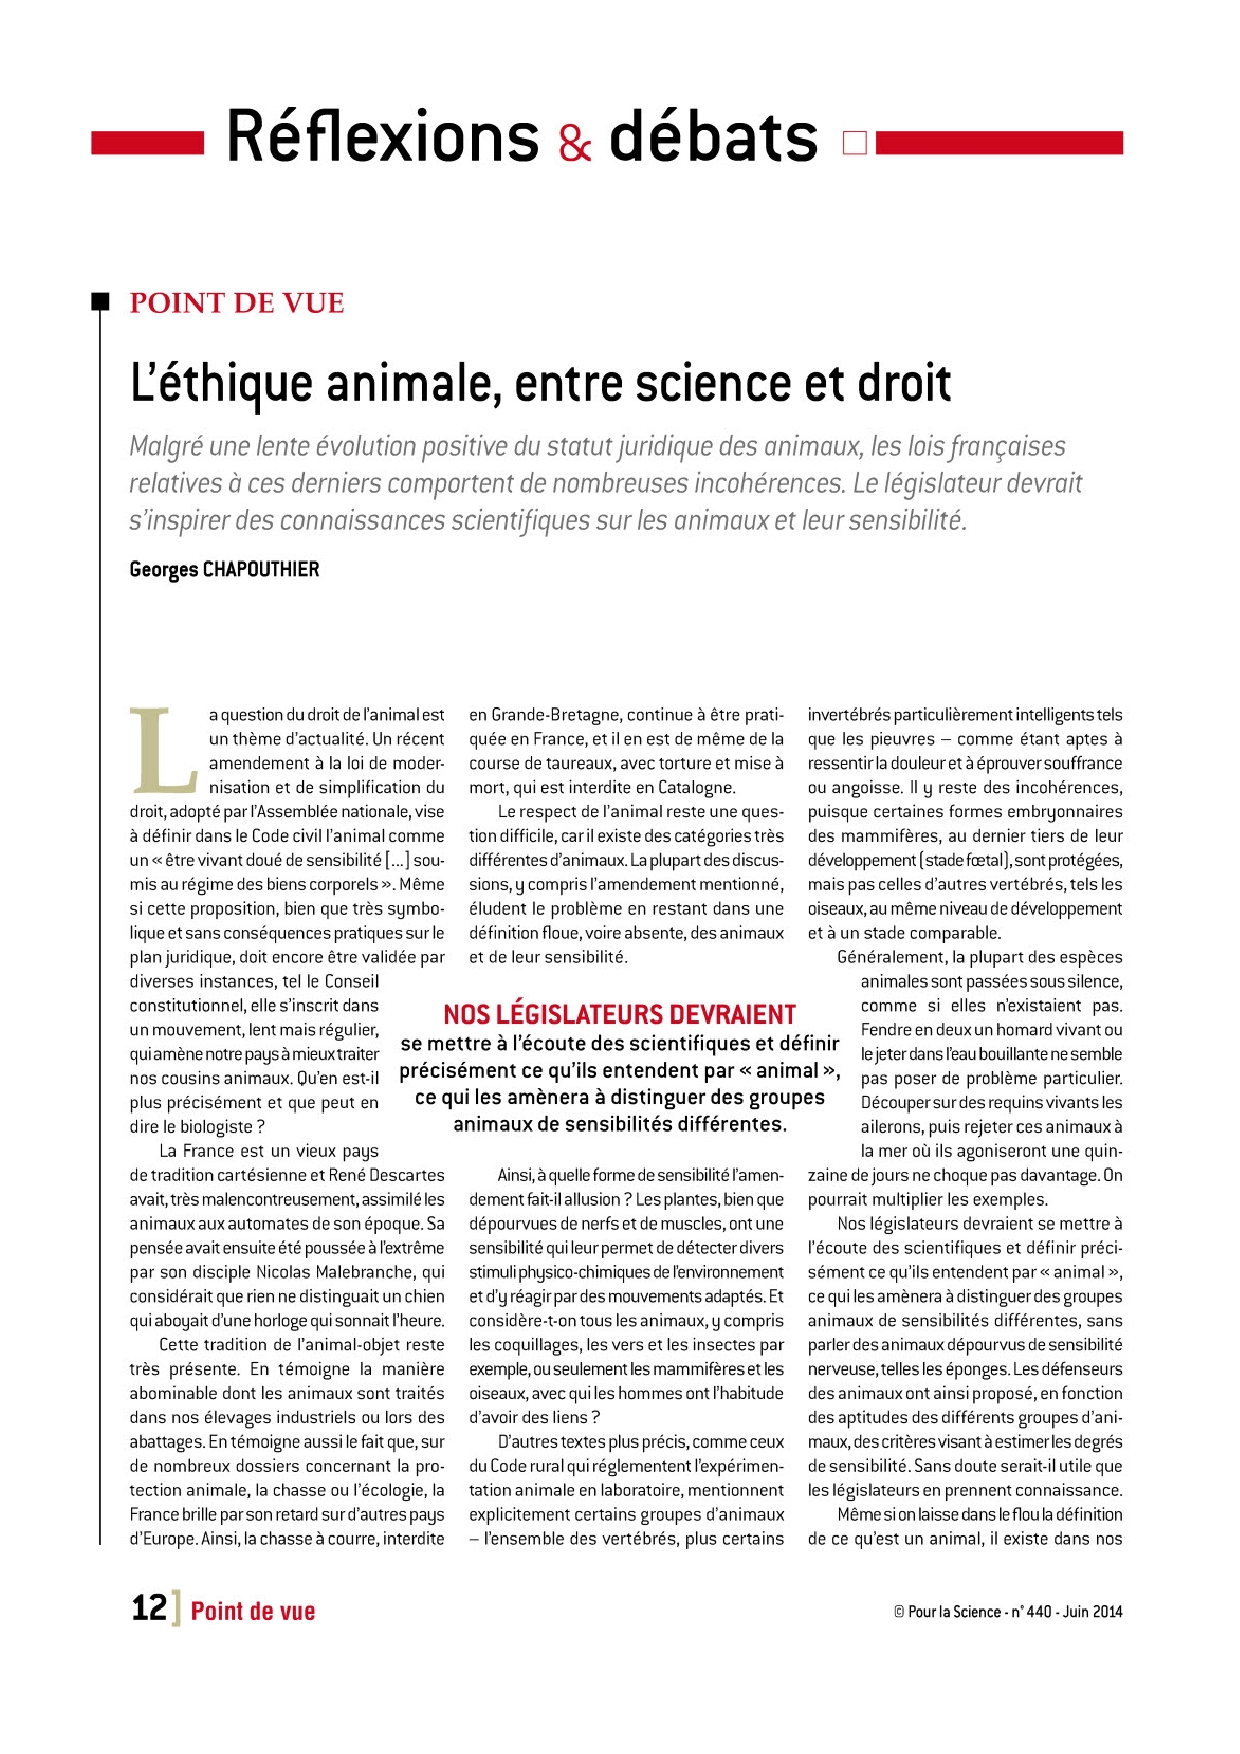
\includepdf[pages=-]{PLS440EthiqueAnimale.pdf}

\end{document}


